% CCZ injection followed by a single teleport with deferred CZ corrections.
% Three registers: |CCZ>, |psi>, |000>.  Same layout and conventions as the
% four-register figure (ccz_teleport): rails numbered top to bottom, Z/X
% meters, classical outcomes m (injection) and t (teleport), and the tracked
% Pauli frame on the output rails.
\documentclass[border=4pt]{standalone}
\usepackage{amsmath,amssymb}
\usepackage{tikz}
\usetikzlibrary{calc,decorations.pathreplacing}

\begin{document}
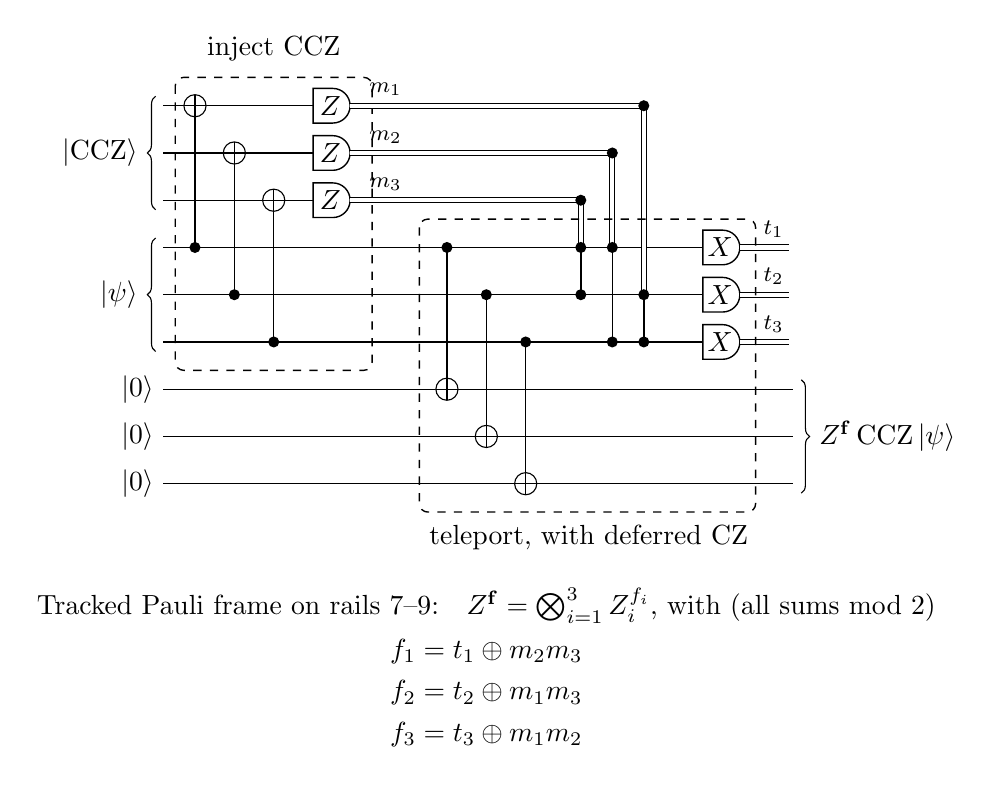
\begin{tikzpicture}[
    x=1cm, y=-0.6cm,
    qw/.style={line width=0.5pt},
    cw/.style={double, double distance=1.5pt, line width=0.4pt},
    ctrl/.style={circle, fill, inner sep=0pt, minimum size=4pt},
    targ/.style={circle, draw, inner sep=0pt, minimum size=8pt, fill=white,
                 path picture={\draw (path picture bounding box.north) -- (path picture bounding box.south)
                                     (path picture bounding box.west)  -- (path picture bounding box.east);}},
    box/.style={draw, dashed, rounded corners=3pt, line width=0.5pt},
    lbl/.style={font=\footnotesize},
  ]

  % ---------------------------------------------------------------- helpers
  % \meter{x}{row}{basis}: D-shaped measurement box, ends at x+0.47
  \newcommand{\meter}[3]{%
    \draw[fill=white, line width=0.5pt] ([shift={(0,0.22cm)}]#1,#2) -- ++(0.25cm,0)
          arc[start angle=90, end angle=-90, radius=0.22cm] -- ++(-0.25cm,0) -- cycle;
    \node[inner sep=0pt] at ([shift={(0.22cm,0)}]#1,#2) {$#3$};}
  % \cnot{x}{control row}{target row}
  \newcommand{\cnot}[3]{%
    \draw[qw] (#1,#2) -- (#1,#3);
    \node[ctrl] at (#1,#2) {};
    \node[targ] at (#1,#3) {};}

  % rows: 1-3 |CCZ>, 4-6 |psi>, 7-9 |0>
  \def\xL{0.3}

  % ---------------------------------------------------------------- quantum wires
  \foreach \r in {1,2,3} \draw[qw] (\xL,\r) -- (2.2,\r);   % CCZ rails up to their meters
  \foreach \r in {4,5,6} \draw[qw] (\xL,\r) -- (7.15,\r);   % psi rails up to their X meters
  \foreach \r in {7,8,9} \draw[qw] (\xL,\r) -- (8.3,\r);   % output rails

  % ---------------------------------------------------------------- input labels
  \draw[decorate, decoration={brace, amplitude=3pt}] (0.2,3.2) -- (0.2,0.8)
        node[midway, left=3pt] {$\lvert\mathrm{CCZ}\rangle$};
  \draw[decorate, decoration={brace, amplitude=3pt}] (0.2,6.2) -- (0.2,3.8)
        node[midway, left=3pt] {$\lvert\psi\rangle$};
  \foreach \r in {7,8,9} \node[left] at (\xL,\r) {$\lvert 0\rangle$};

  % ---------------------------------------------------------------- inject CCZ
  \cnot{0.7}{4}{1}
  \cnot{1.2}{5}{2}
  \cnot{1.7}{6}{3}
  \foreach \r in {1,2,3} \meter{2.2}{\r}{Z};
  \draw[box] (0.45,0.4) rectangle (2.95,6.6);
  \node at (1.7,-0.2) {inject CCZ};

  % classical outcomes m_i, routed to the CZ controls (nested, as in the
  % four-register figure: m_1 outermost, m_3 innermost)
  \draw[cw] (2.67,1) -- (6.4,1) -- (6.4,5);   % m_1 -> CZ(5,6)
  \draw[cw] (2.67,2) -- (6.0,2) -- (6.0,4);   % m_2 -> CZ(4,6)
  \draw[cw] (2.67,3) -- (5.6,3) -- (5.6,4);   % m_3 -> CZ(4,5)
  \node[lbl, above right, xshift=2pt] at (2.72,1) {$m_1$};
  \node[lbl, above right, xshift=2pt] at (2.72,2) {$m_2$};
  \node[lbl, above right, xshift=2pt] at (2.72,3) {$m_3$};

  % ---------------------------------------------------------------- teleport, with deferred CZ
  \cnot{3.9}{4}{7}
  \cnot{4.4}{5}{8}
  \cnot{4.9}{6}{9}

  % classically controlled CZs on the psi rails
  \draw[qw] (5.6,4) -- (5.6,5);  \node[ctrl] at (5.6,4) {}; \node[ctrl] at (5.6,5) {};  % CZ(4,5)^{m_3}
  \draw[qw] (6.0,4) -- (6.0,6);  \node[ctrl] at (6.0,4) {}; \node[ctrl] at (6.0,6) {};  % CZ(4,6)^{m_2}
  \draw[qw] (6.4,5) -- (6.4,6);  \node[ctrl] at (6.4,5) {}; \node[ctrl] at (6.4,6) {};  % CZ(5,6)^{m_1}
  \node[ctrl] at (5.6,3) {}; \node[ctrl] at (6.0,2) {}; \node[ctrl] at (6.4,1) {};      % classical taps

  \foreach \r/\i in {4/1,5/2,6/3} {
    \meter{7.15}{\r}{X};
    \draw[cw] (7.62,\r) -- (8.25,\r);
    \node[lbl, above] at (8.05,\r) {$t_{\i}$};
  }
  \draw[box] (3.55,3.4) rectangle (7.82,9.6);
  \node at (5.7,10.15) {teleport, with deferred CZ};

  % ---------------------------------------------------------------- output
  \draw[decorate, decoration={brace, amplitude=3pt}] (8.4,6.8) -- (8.4,9.2)
        node[midway, right=3pt] {$Z^{\mathbf f}\,\mathrm{CCZ}\,\lvert\psi\rangle$};

  % ---------------------------------------------------------------- Pauli frame
  \node[anchor=north] at (4.4,11.0) {%
    Tracked Pauli frame on rails 7--9:\quad
    $Z^{\mathbf f} = \bigotimes_{i=1}^{3} Z_i^{f_i}$,\ with (all sums mod 2)};
  \node[anchor=north] at (4.4,12.0) {%
    $\begin{aligned}
      f_1 &= t_1 \oplus m_2 m_3 \\
      f_2 &= t_2 \oplus m_1 m_3 \\
      f_3 &= t_3 \oplus m_1 m_2
    \end{aligned}$};
\end{tikzpicture}
\end{document}
